\documentclass[10pt,xcolor=dvipsnames]{beamer}

\usetheme{CambridgeUS}
\setbeamertemplate{footline}[frame number]

\usefonttheme{serif}
\usepackage{pgf,pgfarrows,pgfnodes,pgfautomata,pgfheaps,pgfshade}

\usepackage[english]{babel}
\usepackage{times}
\usepackage{hyperref}
\usepackage{colortbl}
\usepackage{helvet}
\setbeamercovered{dynamic}

\usepackage{beamerthemesplit, natbib, graphicx}
\usepackage{soul}
\usepackage{color}
%\usepackage{biblatex-chicago}

\usepackage{amsmath}
\usepackage{amsfonts}
\usepackage{amssymb}
\usepackage{tikz}

\usepackage[listings]{tcolorbox}
\usepackage{alltt}

\newtheorem{theo}{Theorem}

%\mode<presentation>
%\usetheme{Copenhagen}

\title{
My PhD and Post-Doctoral Research
}

\author{Jing Xu}


\institute{
kenny.xu@duke-nus.edu.sg\\
Centre for Quantitative Medicine, Duke-NUS Medical School, Singapore\\
}


\date{}



\begin{document}



\begin{frame}[plain]
\titlepage
\end{frame}


\begin{frame}[plain]
\frametitle{\color{blue}PhD}
\begin{itemize}
\item 
Proportional hazard model estimation under dependent censoring using maximum penalized likelihood 
\begin{itemize}
\bigskip
\item Brodaty, et al. (2014). Predictors of Institutionalization in Dementia: A three Year Longitudinal Study. Journal of Alzheimer’s Disease.
\bigskip
\item Xu, et al. (2018). Proportional hazard model estimation under dependent censoring using copulas and penalized likelihood. Statistics in Medicine.
\bigskip
\item Xu, J., Ma, J. and Fung, T. (2020). survivalMPLdc: Survival Analysis under Dependent Right Censoring using Maximum Penalised Likelihood. R package version 0.1.0.
\end{itemize}
\end{itemize}
\end{frame}


\frame[plain]
{
\frametitle{\color{blue}Team-PhD}
\begin{itemize}
\item \textbf{Statistic}: Dr Jing Xu, A/Prof Jun Ma, Dr Thomas Fung
\begin{figure}[ht]
\begin{center}
\begin{tabular}{cccc}
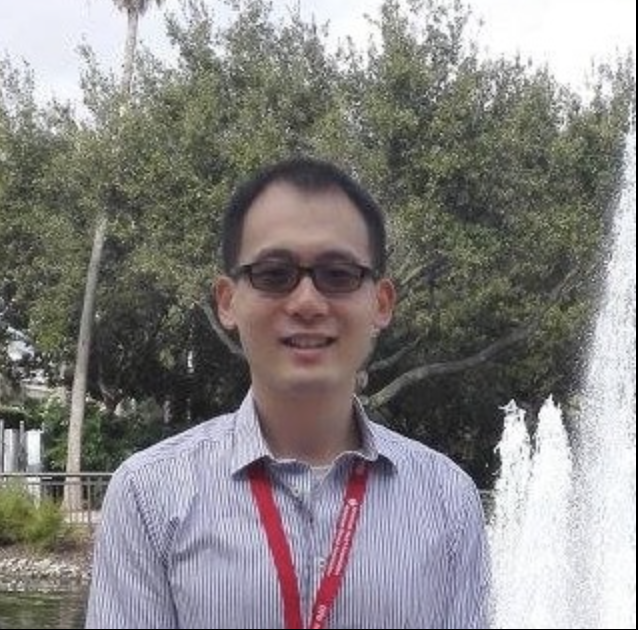
\includegraphics[width=2cm, height=2cm]{Kenny.JPG} &  

\includegraphics[width=2cm, height=2cm]{Jun.JPG} &
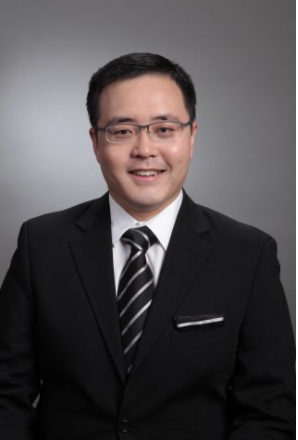
\includegraphics[width=2cm, height=2cm]{Thomas.JPG} &

\includegraphics[width=2cm, height=2cm]{MQ.JPG}  \\
\end{tabular}
\end{center}
\end{figure}
\item \textbf{Medicine}: Dr Michael Connors, Prof Henry Brodaty
\begin{figure}[ht]
\begin{center}
\begin{tabular}{cccc}
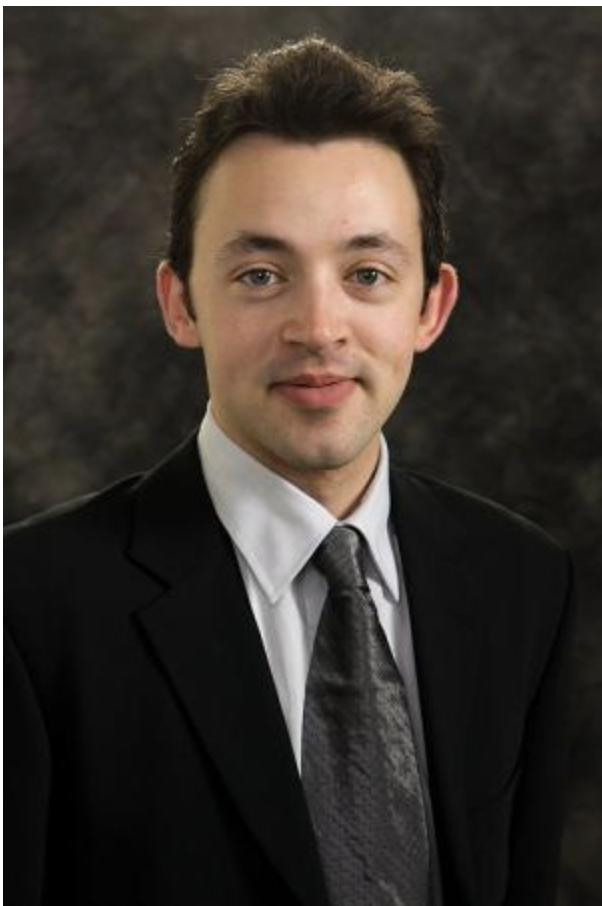
\includegraphics[width=2cm, height=2cm]{Michael.JPG} & 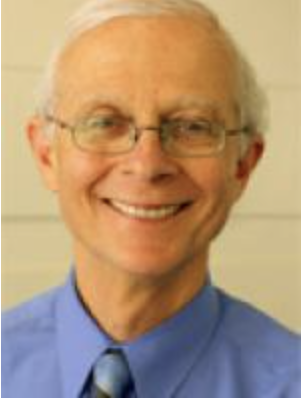
\includegraphics[width=2cm, height=2cm]{Henry.JPG} &  
\includegraphics[width=2cm, height=2cm]{DCRC.JPG} & 
\includegraphics[width=2cm, height=2cm]{UNSW.JPG}\\
\end{tabular}
\end{center}
\end{figure}
\end{itemize}
}

\frame[plain]
{
\frametitle{\color{blue}Postdoc}
\begin{itemize}
\item Multi-Level Micro-Randomized Trial : Detecting the Proximal Effect of Messages on Physical Activity
\bigskip
\begin{itemize}
\item Xu, et al. (2020). Multi-Level Micro-Randomized Trial for Detecting the Proximal Effect of a Mobile Application Messages on Physical
Activity in Diabetes and Depression. arXiv.
\bigskip
\item Aguilera, et al. (2020). An mHealth app using machine learning to increase physical activity in diabetes and depression: clinical trial protocol for the DIAMANTE Study. BMJ Open.
\end{itemize}
\end{itemize}
}


\frame[plain]
{
\frametitle{\color{blue}Team-Postdoc}
\begin{itemize}
\item \textbf{Statistician}: Dr Jing Xu,  A/Prof Bibhas Chackraborty, Miss Xiaoxi Yan \\
\begin{figure}[ht]
\begin{center}
\begin{tabular}{cccc}
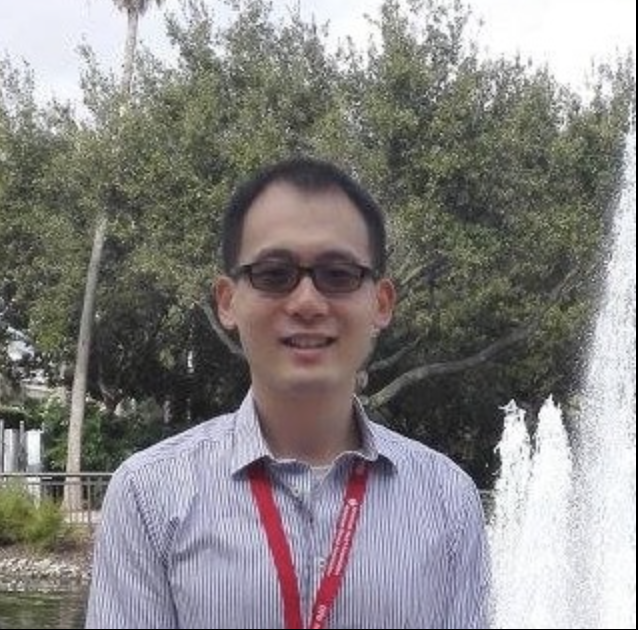
\includegraphics[width=1.5cm, height=1.5cm]{Kenny.JPG} & 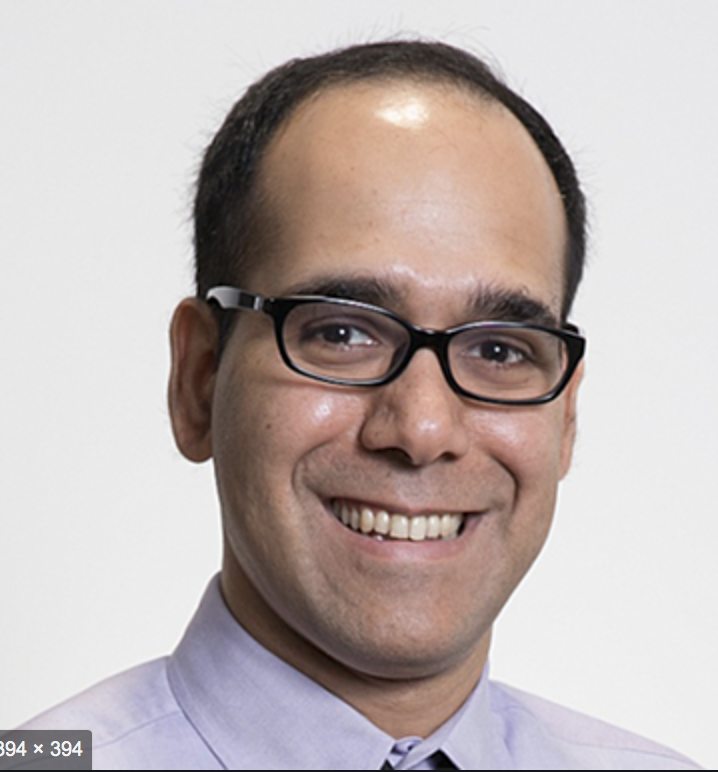
\includegraphics[width=1.5cm, height=1.5cm]{Bibhas.JPG} & 
\includegraphics[width=1.5cm, height=1.5cm]{Xiaoxi.JPG} & 
\includegraphics[width=1.5cm, height=1.5cm]{DUKE-NUS.JPG}\\
\end{tabular}
\end{center}
\end{figure}
\item \textbf{Social Welfare}: A/Prof Adrian Aguilera, Dr Caroline Figueroa\\
\begin{figure}[ht]
\begin{center}
\begin{tabular}{ccc}
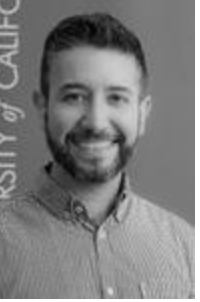
\includegraphics[width=1.5cm, height=1.5cm]{Adrian.JPG} 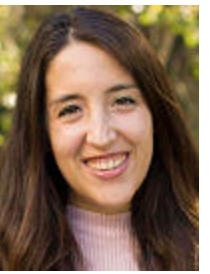
\includegraphics[width=1.5cm, height=1.5cm]{Caroline.JPG} 
\includegraphics[width=1.5cm, height=1.5cm]{UC.JPG}
\end{tabular}
\end{center}
\end{figure}
\item \textbf{Computer Scientist}: Dr Joseph Williams\\
\begin{figure}[ht]
\begin{center}
\begin{tabular}{cc}

\includegraphics[width=1.5cm, height=1.5cm]{Joseph.JPG} 
\includegraphics[width=1.5cm, height=1.5cm]{UOT.JPG}
\end{tabular}
\end{center}
\end{figure}
\end{itemize}
}

\frame[plain]
{
\frametitle{\color{blue}DIAMANTE Study}
\begin{center}
\underline{DIA}betes and \underline{M}ental Health \underline{A}daptive \underline{N}otification \underline{T}racking and \underline{E}valuation: adaptive-learning and clinic-integrated mobile intervention targeting physical activity to manage co-morbid diabetes and depression in low-income, ethnic minority patients served in the San Francisco Health Network
\begin{figure}
\resizebox{3.5in}{2.0in}{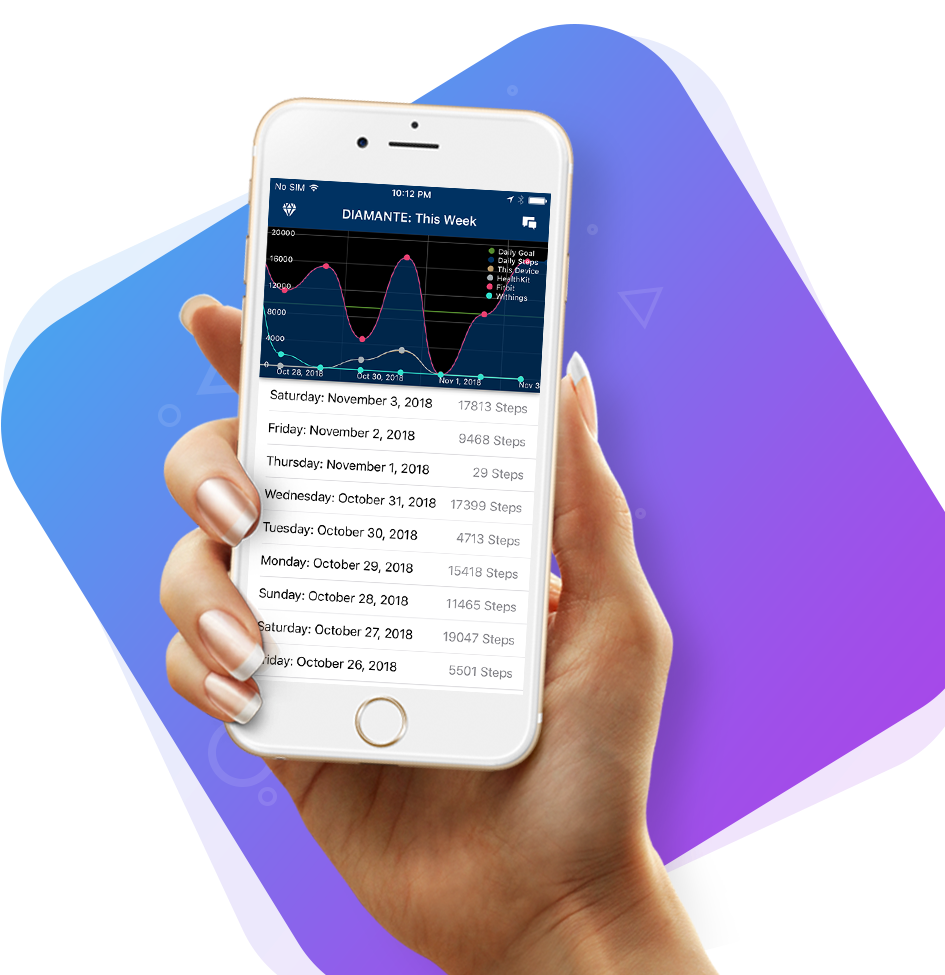
\includegraphics{DIAMANTE_pic.JPG}}
\end{figure}
Source: {\color{blue}https://diamante.healthysms.org/}
\end{center}
}

\frame[plain]
{
\frametitle{\color{blue}Developmental Goal of DIAMANTE Study}
\begin{block}
{2 different messages every day, 1 minute apart}
\begin{figure}
\resizebox{3in}{1.5in}{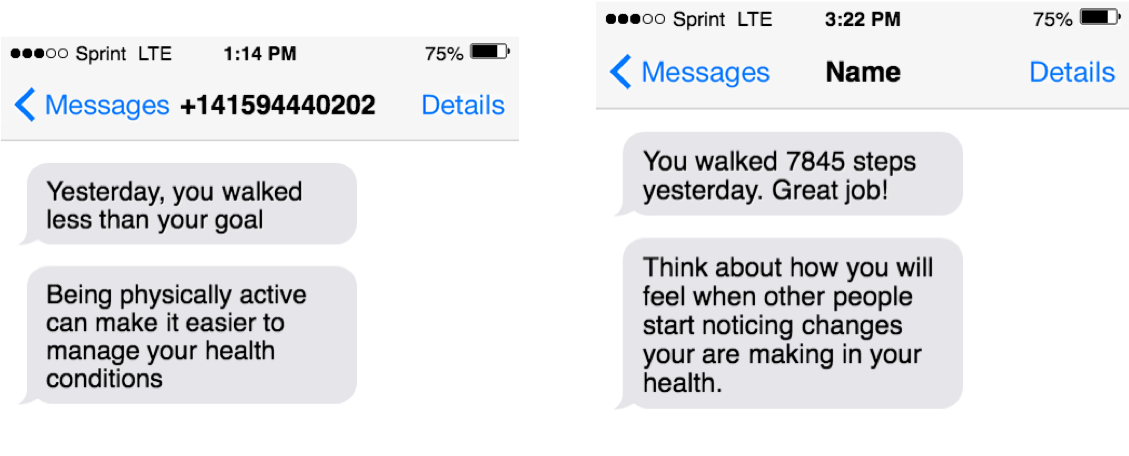
\includegraphics{message-screen.JPG}}
\end{figure}
\end{block}
\begin{itemize}
\item Learn to send better messages to patients to encourage them to walk more 
\item Messages are multi-component interventions, with varying levels of: (a) Time Window (when to send the message), (b) Feedback Message, and (c) Motivational Message
\end{itemize}
}

\frame[plain]
{
\frametitle{\color{blue}Design for DIAMANTE study}
\begin{itemize}
\item The proposed design is called ``Multi-Level Micro Randomized Trial''.
\bigskip
\begin{itemize}
\item It involves multiple message components with more than 2 levels. 
\bigskip
\item For each message component, new levels can be added through the study period. 
\bigskip
\item The possible message levels for each participant are randomized at each sequential decision point.    
\bigskip
\item It captures the ``just-in-time'' adaptive intervention purpose of mobile intervention.
\bigskip
\item Proximal outcome is the walking steps in next 24-hour after a message level sent.
\end{itemize}
\end{itemize}
}


\frame[plain]
{
\frametitle{\color{blue}Analysis Plan}
\begin{itemize}
\item Data structure: longitudinal dataset with time varied interventions
\bigskip
\item Hypothesis test: no proximal effect vs proximal effect exists
\bigskip
\item Analysis type: generalized estimating equations
\bigskip
\item Parameter estimator: least square
\bigskip
\item Test statistics: Chi-squared (Large sample) or Hotelling $t^2$ (small sample)
\end{itemize}

}


\frame[plain]
{
\frametitle{\color{blue}Sample Size Calculation}
\begin{itemize}
\item Power-based:
\smallskip
\begin{itemize}
\item Number of sequential randomization
\smallskip
\item Effect size
\smallskip
\begin{itemize}
\item Initial standardized effect 
\smallskip
\item Average standardized effect  
\smallskip
\item Trend of standardized effect over time  
\end{itemize}
\item Desired power (80\%)
\smallskip
\item Significance level (5\%)
\end{itemize}
\bigskip
\item Precision-based: desired power is replaced by desired coverage probability while effect size is replaced by margin of error.
\end{itemize}
}





\end{document}

